%\section{Facility Location}

%introo  single peak preference and distance function 

\section{Facility Location on the Line}

In this section, we are going to focus on \emph{Facility Location} on the real line. Let $N=\{1,...,n\}$ be the set of agents. Each agent has a private ideal location $x_i\in \mathbb{R}$. We can assume without loss of generality that the locations in the location profile $\x = (x_1, ..., x_n)$ are ordered ($x_1\le x_2\le...\le x_n$), since we focus on anonymous mechanisms. Given an instance $\x$ the most important locations are the leftmost and the rightmost because they delimit the instance. We denote the leftmost location as $lt(\vec{x})=min_{i\in N}\{x_i\}$ and the rightmost location as $rt(\vec{x})=max_{i\in N}\{x_i\}$. The distance function between any two locations is simply the length of the interval, $d(x,y) = |x-y|$. 
%{+??+}


%----------------------------------------------------------------------------
%One facility on the line
\subsection{Locating one facility}

We start with the simplest setting. Given an instance $\x$ we want to place one facility that achieves the best possible social cost in a strategyproof way. 

\begin{theorem}
The mechanism that selects the median location of the reported instance is strategyproof and optimal for the social cost objective.
\end{theorem}

\begin{proof}
We first show that the median location, $med(\vec{x})$, is the optimal solution. If $n$ is odd the median location is $x_{(n+1)/2}$, if $n$ is even any location in the interval $[x_{n/2},x_{n/2+1}]$ is optimal without lost of generality we consider $x_{n/2}$ to be the selected location. Suppose the facility is placed at a location to the left of the median location, let that location be $x$. Then, at least half of the agents' connection cost has increased by $d(x,med(\vec{x}))$, and at most half of the agents' connection cost has decreased by $d(x,med(\vec{x}))$. This makes the social cost of $x$ higher than the optimal. The same holds for any location selected to the right of the median.

We now show that the mechanism is strategyproof. The agent located at $med(\vec{x})$ has no initiative to misreport her location, since her connection cost is zero. Suppose an agent $i$ located at $x_i$ misreports to $x_i'$. Without loss of generality we can assume that $x_i<med(\vec{x})$. If $x_i'<med(\vec{x})$ then the output of the mechanism does not change. If $x_i'>med(\vec{x})$ the median location moves to the right leading to an increase in her cost.
\end{proof}



%------------------------------------------------------------
%Two Facilities on the Line

\subsection{Locating two facilities}
This section extends the previous setting from locating one facility on the real line to locating two. Now a mechanism returns a 2-tuple $\vec{c}=(c_1,c_2)$ with the location of the facilities; we can assume that $c_1 \le c_2$. Each agent connects to the nearest facility with connection cost equal to $cost(x,\vec{c})=min\{ d(x,c_1), d(x,c_2)\}$. 


Let us focus on the optimization problem of locating the two facilities without considering the strategic agents' motives. Let $\vec{x}$ a location profile, and $c_1$,$c_2$ the optimal facility locations.  We can split the agents into two (non-empty) groups based on which facility they prefer. The agents that prefer $c_1$ belong to the "left" set $L(\vec{x})$, and the rest belong to the "right" set $R(\vec{x})$. Using the same argument as in the previous setting for one facility on the line, given the sets $L(\vec{x})$ and $R(\vec{x})$, the optimal locations $c_1$ and $c_2$ are the median of each set. So, for an arbitrary location profile $\vec{x}$, we can compute the optimal solution by selecting the locations that minimize the social cost over the (n-1) choices for $L(\vec{x})$ and $R(\vec{x})$.

%%%????????????????????????
Unfortunately, the mechanism that selects the optimal solution is not strategyproof. The reason is that the sets in the optimal solution are susceptible to minor changes, and the agents can benefit from that. In order to design a strategyproof mechanism we need to extract $L(\vec{x})$ and $R(\vec{x})$ in a strategyproof way. Since both sets are non-empty we are sure that the leftmost agent belongs to $L(\vec{x})$ and the rightmost agent to $R(\vec{x})$. So the mechanism that places the facilities to the leftmost and the rightmost agent is strategyproof and achieves $(n-2)$-approximation ratio. As we will see bellow this is the only deterministic anonymous strategyproof mechanism with bounded approximation for the $2$-Facility Location game. 

\begin{theorem}
The \textsc{Two Extremes} mechanism that places the facilities at the leftmost $lt(\vec{x})$ and the rightmost $rt(\vec{x})$ is a $(n-2)$-strategyproof mechanism for social cost.
\end{theorem}
\begin{proof}
To show the approximation ratio consider the location profile with $n$ agents, where one agent is located at 0, $n-2$ agents are located at $\epsilon>0$ (arbitrarily close to 0), and one agent at 1. The optimal solution places one facility at $\epsilon$ and the other at $1$. The social cost of the optimal solution is $SC^* = \epsilon$. The social cost of the solution outputted by the mechanism is $(n-2)\epsilon = (n-2) SC^*$, since $(n-2)$ agents have connection cost equal to $\epsilon$.

We now show that the mechanism is also strategyproof. Let $\vec{x}$ be a location profile. Any agent reporting a location in the interval $[lt(\vec{x}),rt(\vec{x})]$ cannot change the output of the mechanism. However, if an agent reports a location $x' \in (-\infty,lt(\vec{x})) \cup (rt(\vec{x}),\infty)$ will move the facility further away from her ideal location. So, no agent can benefit by misreporting her location
\end{proof}



%-------------------------------------------------------------------------

In the paper \cite{Procaccia2013} Procaccia and Tennenholtz proved that any deterministic strategy proof mechmanism for 2-Facility Location game has approximation ratio of at least $1.5$. This result was later improved to $2$ \cite{Lu2009}, and then to $(n-1)/2$ \cite{Lu2010} . Fotakis and Tzamos \cite{Fotakis2014} proved a tight lower bound of $n-2$. From the latest result we conclude that the \textsc{Two Extremes} mechanism is the only deterministic, anonymous, strategy-proof mechanism with a bounded approximation ratio.  


The takeaway from the previous section is that we cannot improve the linear approximation ratio for any deterministic strategyproof mechanism. So, the next question is if we can achieve better results with randomized mechanisms. Fortunately, the answer is yes. The \emph{Proportional Mechanism} \cite{Lu2010} is strategyproof and achieves a constant approximation ratio. The idea for this mechanism is very simple and intuitive. Place the first facility uniformly at random among all the reported locations and the second with a probability proportional to its distance from the first. However, is not that simple to prove that the mechanism is indeed strategyproof with constant approximation ratio.

\begin{definition}[Proportional Mechanism]

Given a location profile $\vec{x}=(x_1,...x_n)$, the location of the two facilities are decided by the following random process:
\begin{itemize}
    \item\textbf{Round 1:} Choose agent $i$ uniformly at random from $N$. The first facility $c_1$ is placed at $x_i$

    \item\textbf{Round 2:} Let $d_j = d(c_1,x_j)$ be the distance from agent $j$ to the first facility. Choose agent $j$ with probability $\frac{d_j}{\sum_{k\in N}d_k}$. The second facility is placed at $x_j$.

\end{itemize}
\end{definition}




\begin{theorem}
The proportional mechanism for the two-Facility Location game is strategyproof.
\end{theorem}
\begin{proof}
Let $cost_k(x_i,M(\x))$ denote the expected cost of agent $i$ when the mechanism places the first facility facility on $x_k$. The agent that has a facility at her location experiences after the first round zero cost, so $cost_k(x_k,M(\x))=0$. Since the first facility is selected uniformly at random, we have that for any agent $i$ her total cost is:
\[ cost(x_i,M(\x)) = \frac{1}{n}\sum_{k=1}^{n} cost_k(x_i,M(\x)) = \frac{1}{n}\sum_{k\ne i} cost_k(x_i,M(\x)) \]



Let $\xx=(\x_{i},x_i')$ be the location profile after the deviation of agent $i$. We need to show that she cannot decrease her cost by misreporting her location. We need to show that for all $k\ne i$:

\[ cost(x_i,M(x)) < cost(x_i, M(\xx))\]

Fix the first facility on $x_k$. The expected cost of agent $i$ to the second facility, conditional on the first facility is at $x_k$, is:
\[ cost(c_2,x_i) = \sum_{j=1}^{n} { Pr[c_2=x_j]\cdot d(x_i,x_j)} = \sum_{j=1}^{n} { \frac{d_j}{\sum_{k=1 }^{n}d_k} d(x_i,x_j)}  = \frac{ \sum_{j=1}^{n}d_j \cdot d(x_i,x_j)}{\sum_{j=1}^{n}d_j} \]

Then we have that the cost of agent $i$ is the minimum between the distance to $x_k$ and the expected distance to the second facility:

\begin{align*}
   cost_k(x_i,M(\x)) &= \min\bigg\{d_i, \frac{ \sum_{j=1}^{n}d_j \cdot d(x_i,x_j)}{\sum_{j=1}^{n}d_j}  \bigg\}\\
   &= \frac{\sum_{j=1}^{n}d_j \min\{d_i,d(x_i,x_j)\}}{\sum_{j=1 }^{n}d_j}\\
   &= \frac{\sum_{j\neq i}d_j \min\{d_i,d(x_i,x_j)\}}{\sum_{j=1 }^{n}d_j}
\end{align*}

Let $d_i'=d(c_1,x_i')$. The cost of agent $i$ if she misreports is:
\[ cost_k(x_i,M(\xx)) =\frac{\sum_{j\neq i}d_j \min\{d_i,d(x_i,x_j)\}}{\sum_{j=1 }^{n}d_j + (d_i'-d_i)} + \frac{d_i' \min\{d_i,d(x_i,x_i')\}}{\sum_{j=1 }^{n}d_j + (d_i'-d_i)} \]

We can get the following relation between $cost_k(x_i,M(\x))$ and $cost_k(x_i,M(\xx))$:

\begin{equation}\label{compCost}
cost_k(x_i,M(\xx)) =\frac{ cost_k(x_i,M(\x)) \sum_{j=1}^{n}d_j }{\sum_{j=1 }^{n}d_j + (d_i'-d_i)} + \frac{d_i' \min\{d_i,d(x_i,x_i')\}}{\sum_{j=1 }^{n}d_j + (d_i'-d_i)}    
\end{equation}


We need to distinguish two cases:
\begin{enumerate}[(i)]
    \item $d_i' \le d_i$: we have that $cost_k(x_i,M(\x)) < cost_k(x_i,M(\xx))$ because $\frac{\sum_{j=1}^{n}d_j }{\sum_{j=1 }^{n}d_j + (d_i'-d_i) }>1$ and the second term in the previous equality is non-negative.
    \item $d_i' > d_i$: This case is not that simple. If we subtract $cost_k(x_i,M(\x))$ from (\ref{compCost}), we have:
\[ cost_k(x_i,M(\xx)) - cost_k(x_i,M(\x)) =\frac{ -(d_i'-d_i)cost_k(x_i,M(\x))  }{\sum_{j=1 }^{n}d_j + (d_i'-d_i)} + \frac{d_i' \min\{d_i,d(x_i,x_i')\}}{\sum_{j=1 }^{n}d_j + (d_i'-d_i)}\]

So it suffice to show that:
\begin{equation}\label{s}
   d_i' \min\{d_i,d(x_i,x_i')\}-(d_i'-d_i)cost_k(x_i,M(\x)) \ge 0 
\end{equation}

We need to show that (\ref{s}) holds for both cases:
    \begin{enumerate}
        \item If $\min\{d_i,d(x_i,x_i')\} = d_i$. We have that $d_i \ge cost(x_i,M(\x))$ because agent $i$ always selects the facility closest to her location which cannot be further than the facility placed ad $x_k$. We also have $d_i' \ge d_i' - d_i$. By multiplying the previous inequalities we have that (\ref{s}) holds.
        \item If $\min\{d_i,d(x_i,x_i')\} = d(x_i,x_i')$. We have that $d_i'=d_i \ge cost(x_i,M(\x))$. From triangle inequality we have $d(x_i,x_i') \ge d_i'-d_i$. Again by multiplying the previous inequalities we get that (\ref{s}) holds.
    \end{enumerate}
\end{enumerate}

\end{proof}

It is very interesting that an agent cannot gain even if she knows where the first facility is placed after the first round.

\begin{theorem}
The approximation ratio of the Proportional mechanism for the two Facility Location game is 4 for any metric space.
\end{theorem}

The proportional mechanism is the best know randomized strategyproof mechanism for 2-Facility Location game. The previous know result \cite{Lu2009} has an approximation ratio of $n/2$. A a constant upper bound is a great improvement to the previous liner bound, but there is still a big gap between the upper bound and the only know lower bound for randomized mechanisms, which is $1.045$\cite{Lu2009}. 




\subsection{Locating more than two facilities}

As we previously saw the problem becomes significantly more difficult when we want to locate two facilities instead of one. For the 2-Facility Location games we saw that \textsc{Two Extremes} is the only deterministic and it has a linear approximation ration. Therefore, we cannot expect any better results for $k$-facility location games, when $k\ge3$. In fact we have a very negative result: there is no deterministic anonymous strategyproof mechanism with bounded approximation for $k\ge3$ \cite{Fotakis2014}. This holds even for $n=k+1$ agents. We are going to focus on the intuition behind the proof and present a sketch-proof.  We will refer to deterministic, anonymous, and strategyproof mechanisms with a bounded approximation ratio (in terms of $n$ and $k$) as \emph{nice mechanisms}.



The proof heavily relies at \emph{well-separated instances}, namely instances with $k-1$ isolated agents and two nearby agents. Let $\x = (x_1|x_2|...|x_k, x_{k+1})$ be a well separated instance. The optimal solution is to serve all the isolated agents by a different facility and the two nearby by from the remaining facility. First, we are going to show some properties of nice mechanisms. 

%Given a nice mechanism $M$ with an approximation ration $\rho$ ----- an $a$-approximation mechanism $M$  includes a pair of nearby agents at distance to each other less than $1/a$ times the distance between any other pair of consecutive agents. 


\begin{proposition}
Let $M$ be a nice mechanism for $k$-Facility Location on the line. For any $(k+1)$-location instance $\x$, $M_1(\x) \le x_2$ and $M_k(\x)\ge x_k$
\end{proposition}


\begin{proposition}
Let $M$ be a nice mechanism for $k$-Facility Location. For any $\x=(x_1|x_2|...|x_k,x_{k+1})$ well separated instance, $M_k(\x) \in [x_k,x_{k+1}]$
\end{proposition}

The following propositions show that in well-separated instances if a mechanism places a facility on the left of the nearby agents and we ``push" both agents to the right, while keeping the instance well-separated, the rightmost facility remains on the same agent. Similarly, if a mechanism places a facility on the right of the nearby agents and we ``push" both agents to the left then the rightmost facility remains on the same agent. 

\begin{proposition}
Let $M$ be a nice mechanism for $k$-Facility Location and let  $\x = (x_1|x_2|...|x_k,x_{k+1})$ be a well separated instance such that $M_k(\x) = x_k$. Then for every $\xx = (\x_{-\{k,k+1\}},x_k',x_{k+1}')$ well separated instance with $x_k \ge x_k'$ it holds $M_k(\xx) = x_k'$
\end{proposition}


\begin{proposition} \label{left}
Let $M$ be a nice mechanism for $k$-Facility Location and let  $\x = (x_1|x_2|...|x_k,x_{k+1})$ be a well separated instance such that $M_k(\x) = x_{k+1}$. Then for every $\xx = (\x_{-\{k,k+1\}},x_k',x_{k+1}')$ well separated instance with $x_{k+1} \le x_{k+1}'$ it holds $M_k(\xx) = x_{k+1}'$
\end{proposition}

Using the previous propositions we can show that any anonymous nice mechanism for $k$-facility location on $(k+1)$-agent instances always allocates facilities to the leftmost and to the rightmost agent.

\begin{lemma}\label{leftRight}
Let $M$ be a nice mechanism for $k$-Facility Location with $k\ge2$ and $n=k+1$. Then for all instances $\x=(x_1,...,x_{k+1})$ with $x_1\le...\le x_{k+1}$, $M_1(\x) = x_1$ and $M_k(\x)=x_{k+1}$.
\end{lemma}

We can now show that there is no nice mechanism for $k$-Facility Location when $k\ge3$.

\begin{theorem}
For every $k\ge3$, any deterministic strategyproof mechanism for $k$-Facility Location with $n\ge k+1$ agents on the line has an unbounded approximation ratio. 
\end{theorem}
The previous propositions and the lemma describe how any nice mechanism should ``behave". Suppose that there is a nice mechanism $M$ with a bounded approximation for 3-Facility Location. Let  $\x=(x_1|x_2|x_3,x_4)$ be a well-separated instance. By Lemma \ref{leftRight} $x_1$ and $x_4$ have a facility. And since the instance is well-separated agent $x_3$ is served by the facility at $x_4$. 
\begin{figure}[ht]
    \centering
    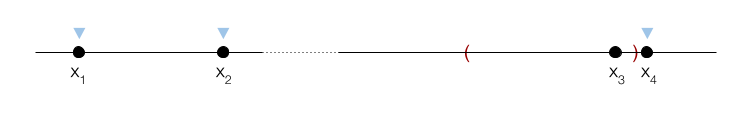
\includegraphics[width=12cm]{Images/imposibility1.png}
    \caption{$\x$}
    \label{fig:imp1}
\end{figure}

Let us remind the definition of the image set (Definition \ref{imageSet}). The image set of an agent $i$ is the set of facilities the agent can obtain by varying her reported location. Any interval in the complement of an image set $I_i(\x_{-i})$ is called a hole. By Lemma \ref{imageSetLemma} we have that the mechanism places a facility at the location in $I_i(\x_{-i})$ nearest to the location of agent $i$. Since agent $x_3$ is not allocated a facility in $\x$ there is a hole in the image set $I_3(\x_{-3})$ around $x_3$. Let $l$ and $r$ be the locations in $I_3(\x_{-3})$ nearest to $x_3$ on the left and on the right.(let the red lines represent the hole). Now consider the location profile $\y = (\x_{-3}, l+\epsilon)$. By Lemma \ref{imageSetLemma} the mechanisms should place a facility at $l$, since $l$ is the nearest location in the image set.


\begin{figure}[ht]
    \centering
    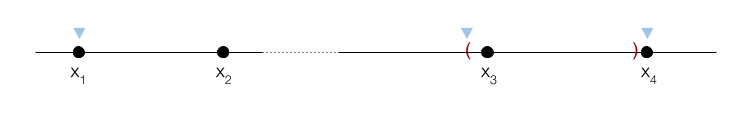
\includegraphics[width=12cm]{Images/imposibility2.png}
    \caption{$\y$}
    \label{fig:imp2}
\end{figure}

Now consider the location profile $\vec{z}=(\y_{-4},l)= (\x_{\{-3,4\}},\{l,l+\epsilon\})$. The mechanism is anonymous, which means we can rearrange the indices so that $x_1\le x_2 \le x_3\le x_4$. As a result, agents 3 and 4 switch indices in $\y$ and $\vec{z}$. We have that $M$ is strategyproof. Since in $\y$ and in $\vec{z}$ there is an agent at $l+\epsilon$ and in $\vec{z}$ an agent is moving closer to $l$, $M$ should keep a facility at $l$. By proposition \ref{left} we have that $x_4$ has a facility because $\x$ and $\vec{z}$ are well-separated instances and the nearby agents move to the right. But this way in $\vec{z}$ the nearby agents are allocated two facilities which makes the cost arbitrarily larger than the optimal.


%In $y$ and $z$ there is an agent at $l+\epsilon$. $M$ is strategyproof and since $M$ places a facility in $y$ at $l$ and in $z$ there is an agent at $l$, $M$ should keep a facility at $l$.
% In $\y$ and in $\vec{z}$ there is an agent at $l+\epsilon$ and in $\vec{z}$ an agent is moving closer to $l$. Since $M$ is strategyproof it should keep a facility at $l$


\begin{figure}[ht] 
    \centering
    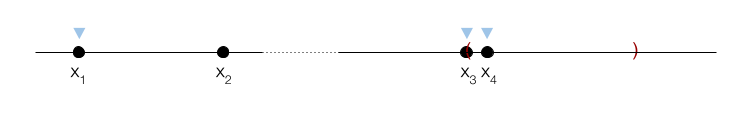
\includegraphics[width=12cm]{Images/imposibility3.png}
    \caption{$\vec{z}$}
    \label{fig:imp3}
\end{figure}



%---------------------------------------------------------------------------
% percentile mechanisms 
Even if we cannot have deterministic strategyproof mechanisms with a bounded approximation ration for the $k$-Facility Location games with $k\ge3$, there is a class of deterministic strategyproof mechanisms \cite{Sui2013}  for any $k\ge2$. A percentile mechanism splits the instance into $k$ parts, based on a predefined vector $\vec{p} \in (0,1)^k$, and allocates one facility at each part. One might think how can this class of mechanisms be practical if there is no guaranty for the outcome. However, in most ``real world" applications the designer has some knowledge of the preferences of the participating agents. This allows for empirical optimization of the vector $\vec{p}$. Let us formally define the percentile mechanisms.

\iffalse
\bigskip
Since we focus on anonymous mechanism we can assume without loss of generality that in an instance $\x = (x_1,...,x_n)$ all the agents' locations are in an ascending order ($x_1\le ... \le x_n$).  
\fi


\begin{definition}[$\vec{p}$-percentile mechanism]
The percentile mechanism is specified by a vector $\vec{p}=(p_1,...,p_k)$ where $0\le p_1\le...\le p_k \le 1$. The mechanism locates $j$th facility at the $p_j$th percentile of the reported locations. 
\[ c_j = x_{i_j}\; :\; i_j = \lfloor (n-1)\cdot p_j \rfloor +1 \]

\end{definition}

To better understand the mechanism let $\x = (x_1,...,x_9)$ be a location profile with $9$ agents. The $(0.25,0.75)$-percentile mechanism will place the first facility at $c_1=x_3$ since $\lfloor 8\cdot 0.25 \rfloor +1  = 3$ and the second facility at $c_2=x_7$ since $\lfloor 8\cdot 0.75 \rfloor +1 = 7$. 


\begin{figure}[ht]
    \centering
    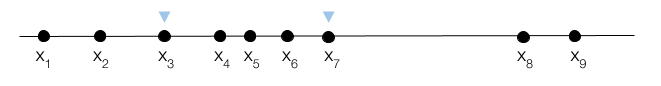
\includegraphics[width=12cm]{Images/percentile.png}
    \caption{Example of $(0.25,0.75)$-percentile mechanism for 9 agents}
    \label{fig:percentileExample}
\end{figure}

\begin{lemma}
The percentile mechanism is group strategyproof for any $\vec{p}$.
\end{lemma}

\begin{proof}
We are going to prove the lemma for $k=2$ but the proof is similar for $k\ge2$. Let $\vec{c}=(c_1,c_2)$ be the locations of the facilities when all the agents report their true preferences and $\vec{c}'=(c_1',c_2')$ be the locations after agents in a subset $S\subset N$ deviate from their true locations. Let $\Delta_1 = c_1-c_1'$ and $\Delta_2 = c_2'-c_2$. Now we need to show that at least one agent in $S$ does not benefit from the deviation. There are four cases to consider:
\begin{enumerate}[(i)]
    \item $\Delta_1\ge0$ and $\Delta_2>0$. That means that the first facility is moved to the left and the second to the right. In order for this to happen there is one agent that has an ideal location $x_i \in (c_1,c_2)$ who reported a location either to the left of $c_1$ or to the right of $c_2$. Otherwise the facilities could not move in such way. Now the cost of agent $i$ is:
    \begin{align*}
        cost(x_i,M(\xx)) &= min(d(x_i,c_1'),d(x_i,c_2'))\\
        &\ge min(d(x_i,c_1),d(x_i,c_2))\\
        &= cost(x_i,M(\x))
    \end{align*}
    \item $\Delta_1\ge0$ and $\Delta_2<0$. Now both facilities moved to the left. That means there is an agent $i$ with $x_i>c_2$, that reported a location to the left of $c_2$. Her cost is:
    \[ cost(x_i,M(\xx)) = x_i -c_2' \ge x_i-c_2 = cost(x_i,M(\x))\]
    \item $\Delta_1<0$ and $\Delta_2\ge0$. This case is completely symmetric to the previous case.
    \item $\Delta_1<0$ and $\Delta_2<0$. The first facility is moved to the right and the second to the left. As in the second case there is an agent to the right of $c_2$ that reported a location to the left. She cannot benefit from this deviation.
\end{enumerate}
Note that if $\Delta_1=0$ and $\Delta_2=0$ represents the case where neither facility moves and no agent benefits from the deviation. So without loss of generality we can assume that at least one of $\Delta_1$ or $\Delta_2$ is non-negative. 

\end{proof}
 
The main idea behind the proof is that the mechanism selects where to open a facility without ``looking" at the instance. Like in the example above in any instance (with $9$ agents) the $(0.25,0.75)$-percentile mechanism  will place the facilities at the $3$nd and $7$th agent respectively without looking at their actual locations. In order for an agent to change the outcome of the mechanism she would have to report a location $x'$ in a different part than her true preference. Like in the setting with one facility (and the median location) this deviation would move the facility further away making it a non profitable deviation. 


The \textsc{Two Extremes} mechanism mention above belongs in the class of percentile mechanism with a vector $\vec{p}=(0,1)$. It is also the only mechanism within the family of percentile mechanisms that has a bounded approximation ratio. For any $\vec{p}\neq (0,1)$ we can create an instance with arbitrarily small cost but since the mechanisms does not ``look" at the instance the solution will have arbitrarily large cost. Consider a location profile $\x=(0,\epsilon,1)$ where $\epsilon>0$ but arbitrarily close to $0$. The $(0,0.6)$- percentile mechanism will allocate the facilities to the first two agents. It is easy to see that the cost of the optimal solution is $\epsilon$ but the cost of the solution of the mechanism is $1-\epsilon$. Thus, the approximation ratio is unbounded.

~\\\textbf{Randomized mechanisms}

%{+Counter-example for proportional for 3 facilities+}
Again we may get better results if we consider randomized mechanism for $k$-Facility Location on the line. Unfortunately, a simple extensions of the proportional mechanism is not strategyproof even when $k=3$. The first two facilities are allocated like in the Proportional mechanism and the third is placed on a location of an agent with probability proportional to her minimal distance to the first two facilities. 

Consider this counter-example: there exist $n_0$ agents at $0$, $n_1$ agents at location $1$, $n_2$ agents at location $1+x$ and 1 agent at location $1+x+y$. Here $n_0$ is sufficiently large such that we can assume the first facility to be always located at $0$. In this configuration, let $y=100$, $x=10^{100}$, $n_1=50$ and $n_2=4$. An agent at location 1 may have the incentive to misreport to location 1+x. 

If we take a closer look at the instance, we can see that the distance between locations 0 and 1 is 1, and between locations $1+x$ and $1+x+y$ is $y$. By selecting $x=10^{100}$, the distance between locations 1 and $1+x$ is huge compared to the other two distances. By construction, the mechanism places the first facility at 0. Since the second facility is placed with a probability proportional to the distance to the first facility, the agent's deviation to $1+x$ increases the probability the second facility is placed at $1+x$. But that also means that the third facility  has an increased probability of being placed  at her true location, making that mechanism manipulable.




%{+Imposing mechanisms+}
Due to the negative results in the general setting new approaches were proposed. Imposing mechanisms was proposed by Nissim, Smorodinsky, and Tennenholtz \cite{Nissim2010}, namely mechanisms able to restrict how agents exploit their outcome. Fotakis and Tzamos \cite{Fotakis2013} showed that the winner-imposing version of the Proportional mechanism is strategyproof for the $k$-Facility Location game, and achieves an approximation ratio of at most $4k$. In this setting any agent that ``wins" a facility at her reported location must connect to it, even if there is a location closer to her ideal location. The mechanism runs in $k$ rounds and allocates one facility at each round. For each $\ell=1,...,k$ let $C_\ell$ denote the facility set after the $\ell$th round. 


\begin{definition}[Winner Imposing Proportional Mechanism]

Given a location profile $\vec{x}=(x_1,...x_n)$, the mechanism runs the following random process:
\begin{itemize}
    \item\textbf{Round 1:} Choose agent $i$ uniformly at random from $N$. The first facility is placed at $x_i$. Let $C_1=\{x_i\}$

    \item\textbf{Round $\ell$}, $\ell = 2,...,k$: Let $d_\ell = d(x_\ell,C_{\ell-1})$ be the distance from agent $\ell$ to the closest facility. Choose agent $\ell$ with probability $\frac{d_\ell}{\sum_{k\in N}d_k}$. The $\ell$th facility is placed at $x_\ell$, and agent $x_\ell$ connects to it. Let $C_\ell=C_{\ell-1}\cup \{x_\ell\}$

\end{itemize}
\end{definition}


%\subsubsection{Conclusion}

%conclution && different settings
%{+Equal cost?+}
%{?Verification?}
